\subsection{Smart Pixels for LHC}
{{\footnotesize
\noindent Presents a 256x256-pixel ROIC in 28 nm CMOS with embedded 2-layer NN for cluster filtering
at 25 ns, achieving 54-75\% data reduction while maintaining noise and latency constraints. Prototype
consumes \textasciitilde{}300 microW/pixel and operates in combinatorial digital logic.


\begin{description}[labelwidth=4cm, labelsep=1em, leftmargin=4cm, itemsep=0.1em, parsep=0em]
  \item[date:] 2024-06-24
  \item[version:] v1.0
  \item[last\_updated:] 2024-06
  \item[expired:] unknown
  \item[valid:] yes
  \item[valid\_date:] 2024-06-24
  \item[url:] \href{https://arxiv.org/abs/2406.14860}{https://arxiv.org/abs/2406.14860}
  \item[doi:] 10.48550/arXiv.2406.14860
  \item[domain:]
    - High Energy Physics
  \item[focus:] On-sensor, in-pixel ML filtering for high-rate LHC pixel detectors
  \item[keywords:]
    - smart pixel
    - on-sensor inference
    - data reduction
    - trigger
  \item[licensing:] Via Fermilab
  \item[task\_types:]
    - Image Classification
    - Data filtering
  \item[ai\_capability\_measured:]
    - On-chip
    - low-power inference; data reduction
  \item[metrics:]
    - Data rejection rate
    - Power per pixel
  \item[models:]
    - 2-layer pixel NN
  \item[ml\_motif:]
    - Classification
  \item[type:] Benchmark
  \item[ml\_task:]
    - Image Classification
  \item[solutions:] Solution details are described in the referenced paper or repository.
  \item[notes:] Prototype in CMOS 28 nm; proof-of-concept for Phase III pixel upgrades.

  \item[contact.name:] Lindsey Gray; Jennet Dickinson
  \item[contact.email:] unknown
  \item[results.links.name:] ChatGPT LLM
  \item[fair.reproducible:] Yes
  \item[fair.benchmark\_ready:] Yes (Zenodo:7331128)
  \item[id:] smart\_pixels\_for\_lhc
  \item[Citations:] \cite{parpillon2024smartpixelsinpixelai}
\end{description}

{\bf Ratings:} ~ \\

\begin{tabular}{p{0.15\textwidth} p{0.07\textwidth} p{0.7\textwidth}}
\hline
Rating & Value & Reason \\
\hline
dataset & 2 & No dataset links; not publicly hosted or FAIR-compliant
 \\
documentation & 3 & Paper contains detailed descriptions, but no repo or external guide for reproducing results
 \\
metrics & 5 & None
 \\
reference\_solution & 3 & In-pixel 2-layer NN described and evaluated, but reproducibility and source files are not released
 \\
software & 2 & No packaged code or setup scripts available; replication depends on hardware description and paper
 \\
specification & 5 & None
 \\
\hline
\end{tabular}

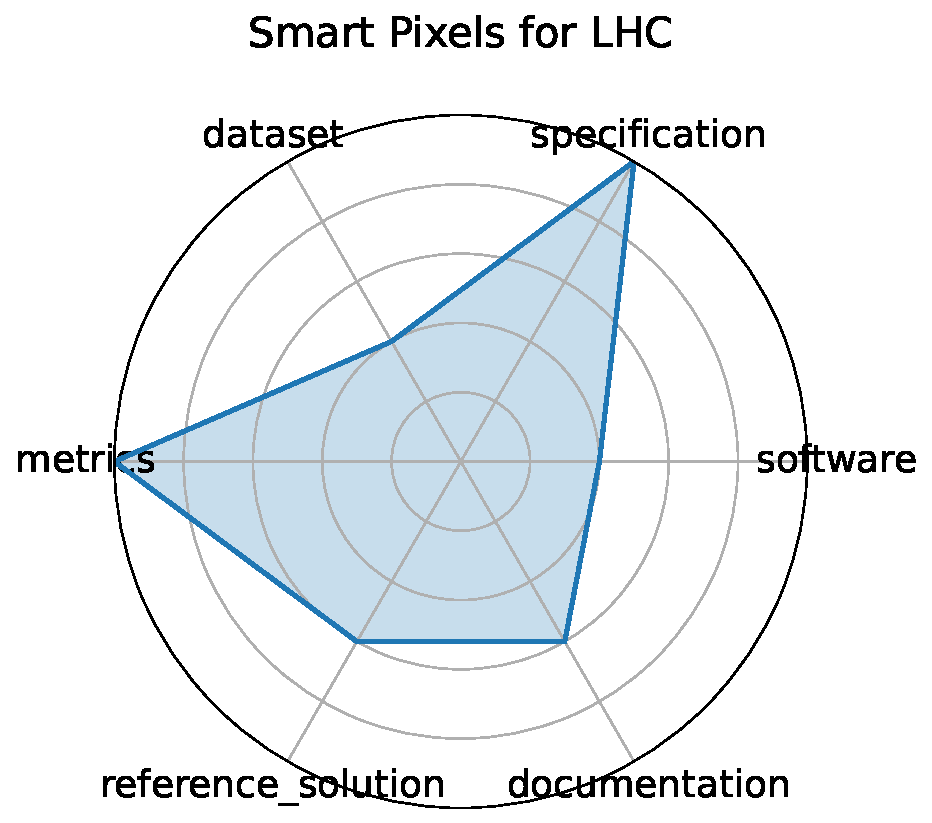
\includegraphics[width=0.2\textwidth]{smart_pixels_for_lhc_radar.pdf}
}}
\clearpage